\documentclass[11pt,aspectratio=169]{beamer}
\usetheme{CambridgeUS}
\beamertemplatenavigationsymbolsempty
\usepackage{fontspec}
\setsansfont{Junicode}
\usepackage{amsmath,mathtools}
\usepackage{hyperref}
\usepackage{graphicx}
\usepackage{xpatch}
\usepackage[export]{adjustbox}
\usepackage{pgfplots}
\usepackage{tikz}

\usetikzlibrary{shapes,calc,matrix,decorations.markings,decorations.pathreplacing,positioning, intersections,backgrounds,through,hobby,arrows.meta}
\usepackage{csquotes}
\usepackage[french]{babel}
\date[10/09/2024]{Nancy, 10 septembre 2024}
\author[Matthias \textsc{Gille Levenson}]{Journées d'Études \enquote{De la transcription manuelle participative des textes à la reconnaissance automatique de texte (ATR/HTR) : outils, théorie, pratiques.}\\~\\ Matthias \textsc{Gille Levenson}\\   {\scriptsize École Nationale des chartes -- Centre Jean Mabillon \& École Normale Supérieure de Lyon - CIHAM UMR 5648}\vspace{-.5cm}%\\ {\tiny prénom [point] gille [tiret] levenson [at] ens-lyon [point] org}\vspace{-.5cm}%
}
\title[De la donnée avant toute chose?]{De la donnée avant toute chose? Retour d'expérience de l'utilisation de l'HTR dans des projets d'édition et d'étude des textes médiévaux}
\titlegraphic{\vspace{-.5cm}\includegraphics[scale=0.18]{/home/mgl/Bureau/Travail/admin/logos/enc.png}\hspace{0.5cm}\includegraphics[scale=0.18]{/home/mgl/Bureau/Travail/admin/logos/ensl.png}\hspace{0.5cm}\includegraphics[scale=0.20]{/home/mgl/Bureau/Travail/admin/logos/logo-ciham.png}}


%\usepackage[labelformat=empty]{caption}
\setbeamertemplate{caption}{\insertcaption\par}

\usepackage[datamodel=thesis,citestyle=authoryear,isbn=true,
doi=true,backend=biber,language=french,url=true,sorting=nty,maxnames=6, maxcitenames=4]{biblatex}
\renewbibmacro{in:}{}
\renewcommand*{\bibfont}{\tiny} 
% http://mcclinews.free.fr/latex/introbeamer/elements_contenu.html
%\xapptobibmacro{cite}{\setunit{\nametitledelim}\printfield{year}}{}{}
\addbibresource{/home/mgl/Bureau/These/Edition/hyperregimiento-de-los-principes/Dedans/XML/corpus/biblio.bib}

\begin{filecontents*}{thesis.dbx}
\ProvidesFile{thesis.dbx}[2014/06/14 supervisor for theses]
\RequireBiber[3]
\DeclareDatamodelFields[type=list,datatype=name]{supervisor}
\DeclareDatamodelEntryfields[thesis]{supervisor}
\end{filecontents*}


\begin{filecontents*}{french-thesis.lbx}
\ProvidesFile{french-thesis.lbx}[2014/06/14 english for thesis]
\InheritBibliographyExtras{french}
\NewBibliographyString{supervision,jointsupervision}
\DeclareBibliographyStrings{%
inherit           = {french},
supervision       = {{dirigée par}{dir\adddotspace }},
jointsupervision  = {{codirigée par}{codir\adddotspace }},
}
\end{filecontents*}

\DeclareLanguageMapping{french}{french-thesis}

\newbibmacro*{thesissupervisor}{%
  \ifnameundef{supervisor}{}{%
    \ifnumgreater{\value{supervisor}}{1}
      {\bibstring{jointsupervision}}
      {\bibstring{supervision}}
    \printnames{supervisor}}}

\xpatchbibdriver{thesis}
  {\printfield{type}}
  {\printfield{type}
   \newunit
   \usebibmacro{thesissupervisor}}
  {\typeout{yep}}
  {\typeout{no}}
  
% https://tex.stackexchange.com/a/184878 ajout direction thèse





\AtBeginSection[]
{\begin{frame}
 \frametitle{}  
 \tableofcontents[currentsection,
                  hideothersubsections,
                  subsubsectionstyle=show/show/show/hide
                   ]
 \end{frame} 
 }



\setbeamertemplate{sections/subsections in toc}[square]
\setbeamertemplate{bibliography item}[sqare]
\setbeamertemplate{itemize item}[square]
\setbeamertemplate{enumerate item}[square]
\setbeamertemplate{itemize subitem}[square]





\renewcommand*{\dotFFN}{}
\newcommand{\astfootnote}[1]{%
\let\oldthefootnote=\thefootnote%
\setcounter{footnote}{0}%
\renewcommand{\thefootnote}{\fnsymbol{footnote}}%
\footnote{#1}%
\let\thefootnote=\oldthefootnote%
}








\setbeameroption{show notes on second screen=right}
\setbeamerfont{note page}{size=\footnotesize}
\addtobeamertemplate{note page}{\setbeamerfont{itemize/enumerate subbody}{size=\tiny}}{}

\begin{document}
\maketitle





\begin{frame}
\frametitle{Plan} % Table of contents slide, comment this block out to remove it
\tableofcontents % Throughout your presentation, if you choose to use \section{} and \subsection{} commands, these will automatically be printed on this slide as an overview of your presentation
\end{frame}


\section{Introduction}
\begin{frame}{Expériences personnelles avec l'HTR}

\begin{itemize}
\item Pour de l'édition
\item Pour l'étude proprement dite du texte
\item Actuellement, pour des expériences de collation multilingue
\end{itemize}

\end{frame}

\begin{frame}{Édition critique}
\begin{figure}
\includegraphics[width=1\textwidth]{img/base_a.png}
\caption{Édition critique du \textit{Regimiento de los Prínçipes}, avec collation automatisée. Les témoins A et Z sont issus d'HTR.}
\end{figure}
\end{frame}


\begin{frame}{Études des marques de lecture d'un manuscrit}
\begin{figure}
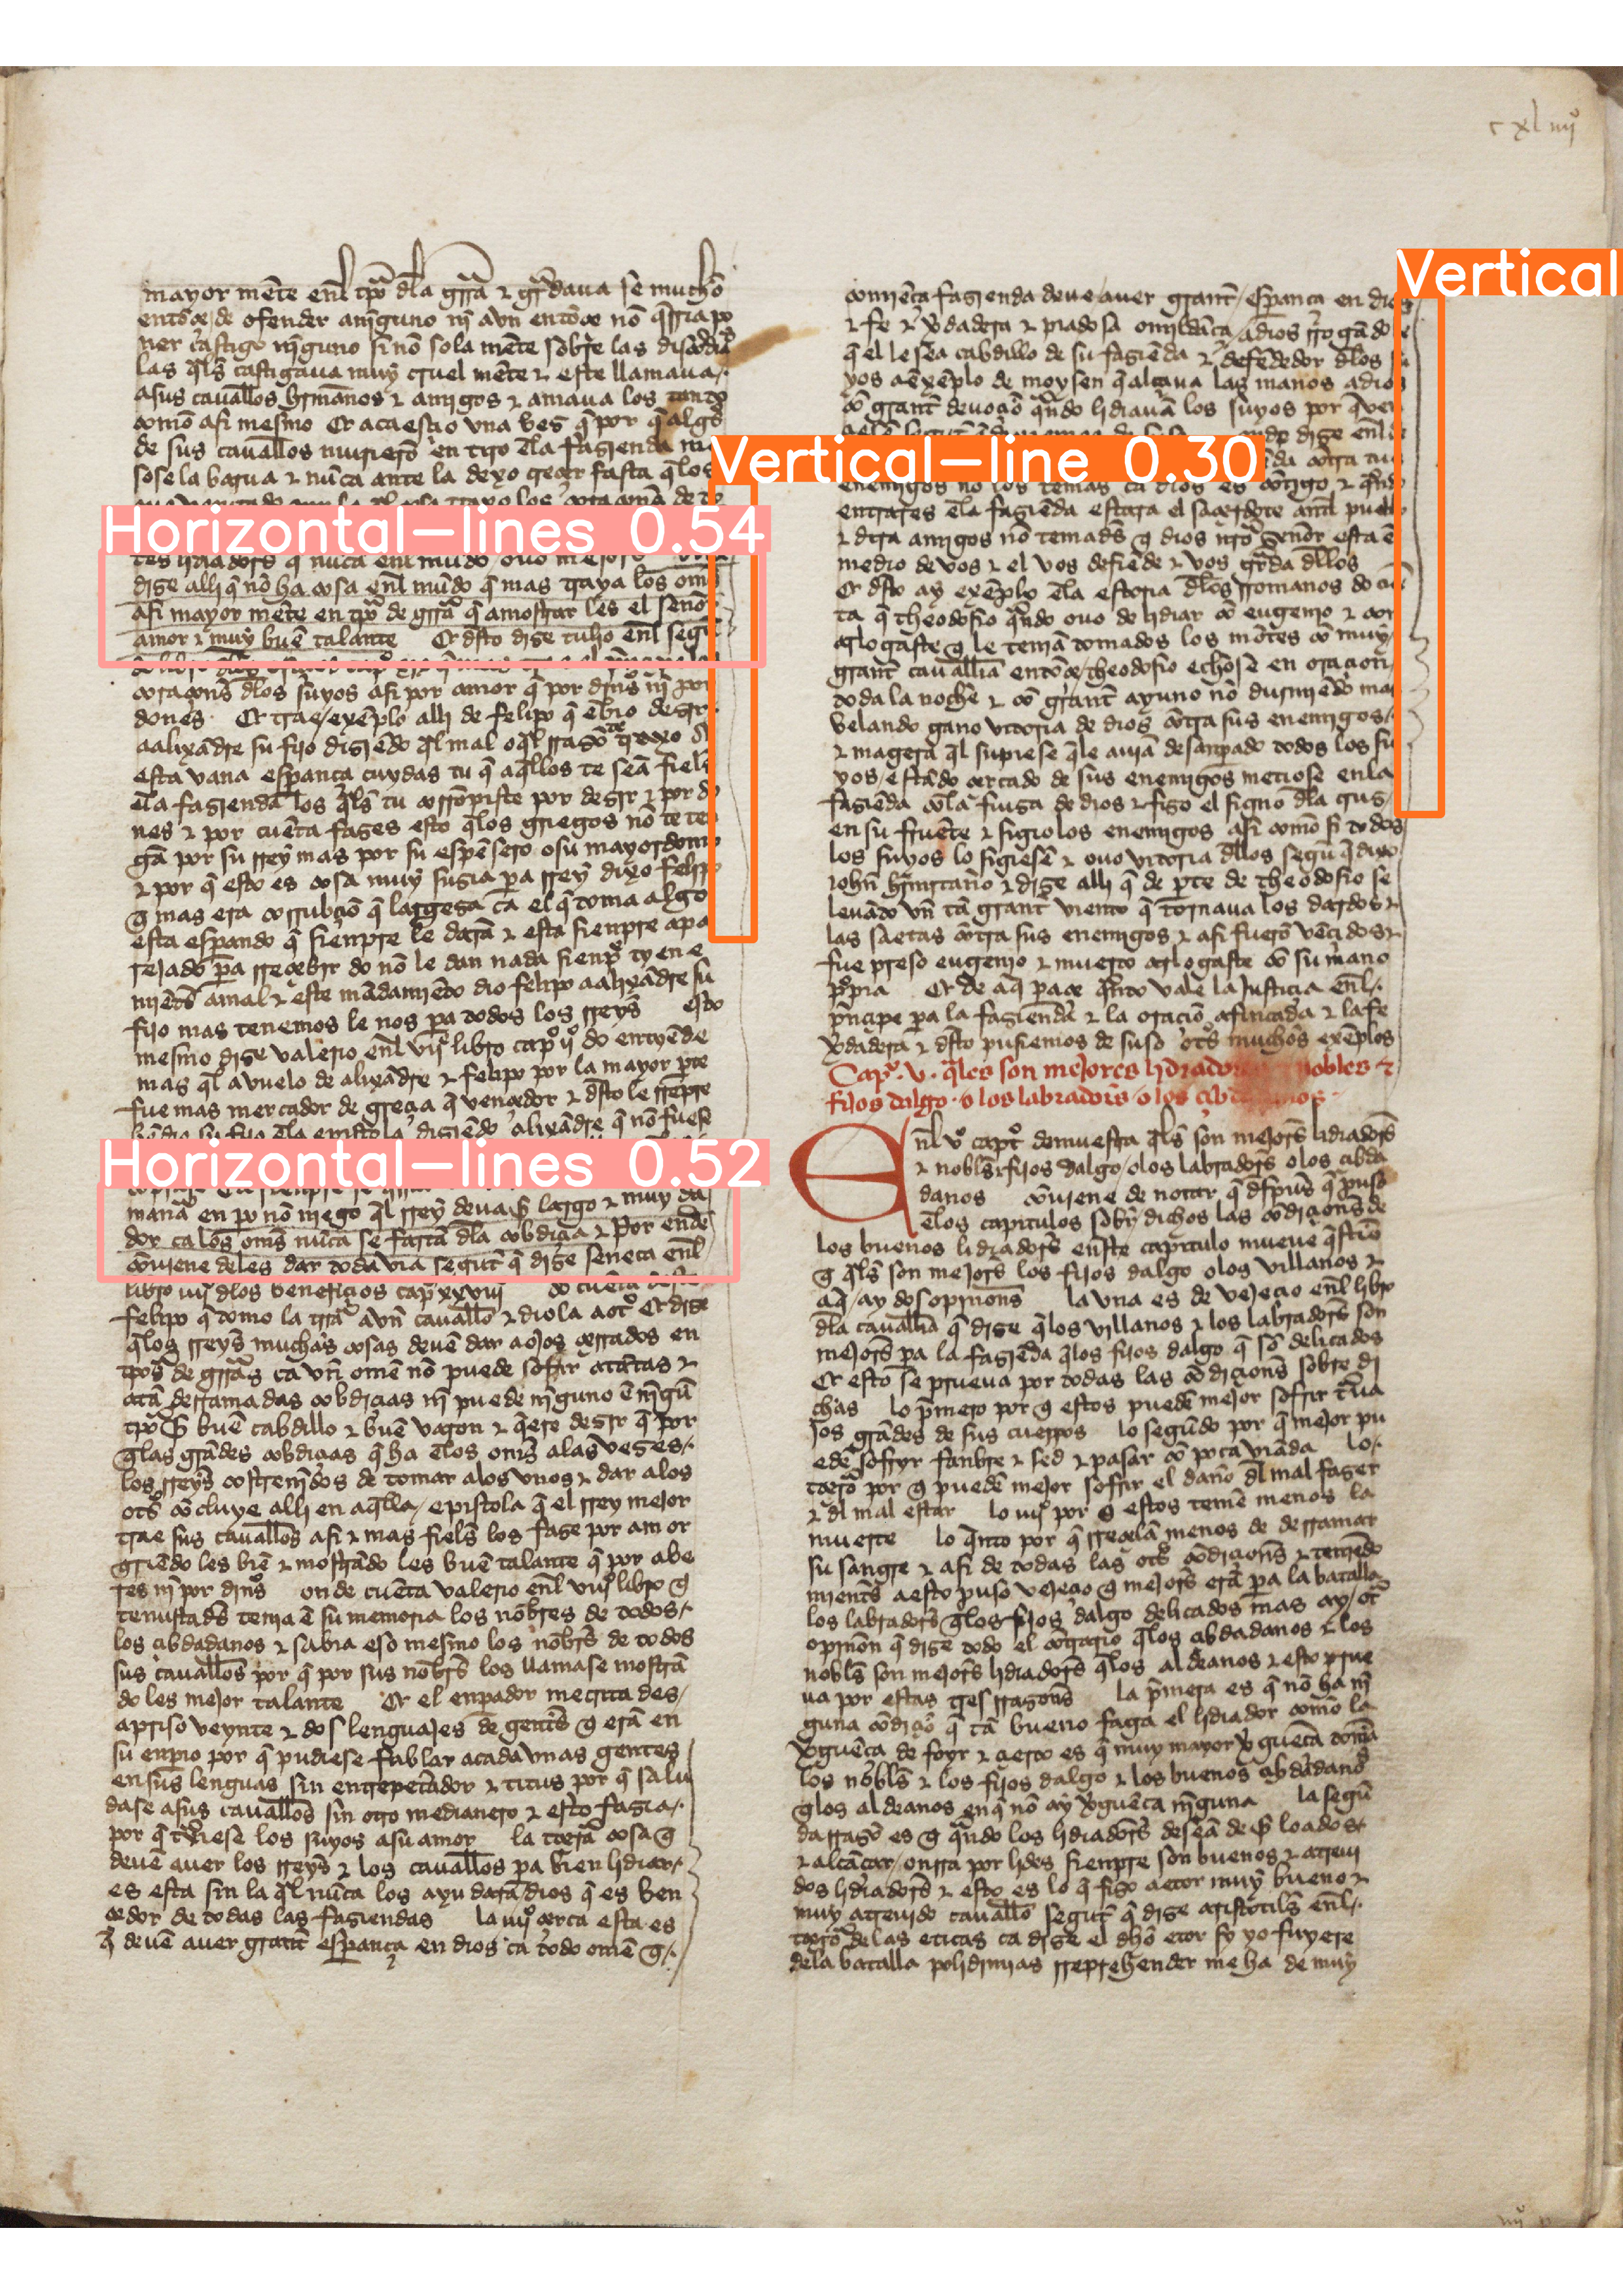
\includegraphics[width=.5\textwidth, trim={0 53cm 0 5cm}, clip]{img/YOLO_identification.png}
\caption{Identification automatisée  (avec YOLO v5) de zones de texte marquées par un lecteur. Escorial Ms. K.I.5, fol. 144r}
\end{figure}
\end{frame}


\begin{frame}{Rappels sur le fonctionnement (actuel) de l'HTR}

\begin{itemize}
\item Trois phases distinctes: segmentation en \textbf{zones}, segmentation en \textbf{lignes}, \textbf{transcription}
\pause\item Respecter les phases et bien découper le travail permet de gagner du temps in fine
\pause\item Avec Kraken, pas de transcription globale du texte mais ligne par ligne pour l'instant
\end{itemize}
\end{frame}

\section{Phase de production des données}

\subsection{Penser la production en amont}

\begin{frame}
\begin{itemize}
\item Différencier et hiérarchiser données et modèles et privilégier les premières sur les seconds
\pause\item Se mettre d'accord en amont de la production (ou via des campagnes d'annotation-test) sur des normes d'annotation (manuel?):

	\begin{itemize}
	\pause\item Quelle typologie des zones et des lignes utiliser ? Identifier les titres de section ?
	\pause\item Que faire des abréviations ?
	\end{itemize}
\end{itemize}
\end{frame}


\subsection{CATMuS, un projet de production collaboratif de données}

\begin{frame}
\begin{itemize}
\item Volonté autour de 2022 de réunir des producteur.ices de données (philologues) venant d'horizons distincts
\item Naissance du projet CATMuS
\end{itemize}
\end{frame}


\begin{frame}{Statistiques sur le corpus CATMuS}
\begin{itemize}
\item Test
\end{itemize}
\end{frame}

\subsection{Concilier l'intérêt particulier et les besoins généraux}

\begin{frame}{Le problème des abréviations, entre usages historiens et usages philologiques}

\end{frame}


\begin{frame}{Le choix de la conservation des abréviations}
\begin{center}



\end{center}
\end{frame}

\section{Après l'HTR: tout change / rien ne change}

\subsection{Quand s'arrête la correction ?}
\begin{frame}
\begin{center}
\begin{itemize}
\item La phase suivant la transcription automatisée sera généralement celle de la transformation en TEI
\item Il restera des erreurs dans les données
\item Faut-il intégrer ces correction dans les données d'entraînement ? 
\item Si oui, cela suppose de penser en amont une modélisation en TEI qui soit rétroconvertible
\item En d'autres termes, il faudra conserver un premier état de TEI diplomatique (qui garde les \texttt{tei:lb})
\end{itemize}
\end{center}
\end{frame}


\begin{frame}{Assurer la rétroconvertibilité ?}
\begin{center}
\begin{figure}
\includegraphics[width=1\textwidth]{img/tei_retroconvertible.png}
\caption{Le document TEI avec des identifiants présents dans le fichier ALTO originel}
\end{figure}
\end{center}
\end{frame}


\begin{frame}{Assurer la rétroconvertibilité ?}
\begin{center}
\begin{figure}
\includegraphics[width=1\textwidth]{img/alto.png}
\caption{Le fichier ALTO en question}
\end{figure}
\end{center}
\end{frame}


\subsection{Structurer les documents}
\begin{frame}{Structurer les documents}
\begin{center}
\begin{itemize}
\item Classifier les zones et les lignes lors de la phase d'ATR peut permettre de faciliter la structuration du document:
\begin{figure}
\includegraphics[width=.45\textwidth]{img/segmentation_lignes.png}
\caption{Classification des lignes suivant le vocabulaire contrôlé SegmOnto. En fuchsia: les lignes de type \texttt{DefaultLine}; en jaune, les lignes de type \texttt{Headingline:rubric}}
\end{figure}
\end{itemize}
\end{center}
\note{
\vfill
L'exemple donné ici est doublement problématique: le numéro de chapitre est erronné, ce qui peut poser problème si l'on utilise le texte pour numéroter les divisions; en second lieu, l'ordre des lignes est évident pour l'humain mais plus difficile à identifier pour la machine, ce qui peut de même poser problème pour la structuration du texte.
\vfill
}
\end{frame}


\subsection{Segmenter le texte et identifier la césure}
\begin{frame}
\begin{center}
\begin{itemize}
\item Dans les manuscrits médiévaux la césure à la ligne n'est pas systématiquement indiquée
\item La tâche d'identification de la césure est raisonnablement automatisable
\end{itemize}
\begin{figure}
\includegraphics[width=.33\textwidth]{img/Valladolid_251_17r.png}
\includegraphics[width=.33\textwidth]{img/Borgh_360_190r.png}
\includegraphics[width=.33\textwidth]{img/CCC_MSS_283_14r.png}
\includegraphics[width=.33\textwidth]{img/Valencia_BH-Ms-0594_23r.png}
\caption{Valladolid, 251 fol. 17r; Vatican, Borgh. 360, fol. 190r; Cambridge, Corpus Christi College, MS 283, fol 14r; Valencia BH Ms 0594, fol. 23r}
\end{figure}
\end{center}
\note{
\vfill
\begin{itemize}
\item On montre des cas d'indications, des cas de non-indication (un texte en castillan, trois en latin; deux manuscrits ibériques, un manuscrit anglais, et un manuscrit italien).
\item Dans le corpus manuscrit castillan du 15e siècle, c'est assez peu commun, alors que l'indication sera plus fréquente en latin par exemple. 
\item Cette tâche ne peut être actuellement efficacement traitée par les outils d'ATR comme Kraken, étant donné que l'outil ne fonctionne que ligne par ligne sans contexte.
\end{itemize}
 
\vfill
}
\end{frame}

\begin{frame}{Segmenter le texte et identifier la césure}
\begin{figure}[htp!]
\begin{center}
\includegraphics[width=0.5\textwidth]{img/ligne_1.png}
\includegraphics[width=0.5\textwidth]{img/ligne_2.png}
\caption{Ms. 251, Valladolid, fol. 3v}
\end{center}
\end{figure}
\begin{quote}
\begin{center}
\pause\textit{adios ⁊ ganaran gloria perdurable ¶ Et pu\\
es que asy es los bienes departen se en una ma}
\end{center}
\end{quote}
\begin{center}
\pause{\color{black}$\Updownarrow$}
\end{center}
\begin{quote}
\begin{center}
\pause\textit{adios ⁊ ganaran gloria perdurable ¶ Et \underline{pues} que asy es los bienes departen se en una ma}
\end{center}
\end{quote}
\note{
\vfill
Il suffit donc d'associer deux à deux les lignes (faire des bigrames de lignes) afin d'identifier si la chaîne de caractère de fin de ligne correspond aussi à une fin de mot.
\vfill
}
\end{frame}

\subsection{Résoudre les abréviations}
\begin{frame}{Résoudre les abréviations}
\begin{center}

\end{center}
\end{frame}


\subsection{Et l'édition critique ?}

\begin{frame}{Et l'édition critique ?}
\begin{center}
\begin{figure}
\includegraphics[width=1\textwidth]{img/avant_correction.png}
\caption{Table d'alignement avant la phase de correction, après segmentation et résolution des abréviations. Gilles de Rome, \textit{De Regimine Principum}, chapitre 1.2.2}
\end{figure}
\end{center}
\note{
\vfill
Un texte difficilement exploitable, en sortie d'HTR désabrévié.
\vfill
}
\end{frame}

\begin{frame}{Et l'édition critique ?}
\begin{center}
\begin{figure}
\includegraphics[width=1\textwidth]{img/apres_correction.png}
\caption{Table d'alignement après la phase de correction. Gilles de Rome, \textit{De Regimine Principum}, chapitre 1.2.1}
\end{figure}
\end{center}\note{
\vfill
\begin{itemize}
\item Il reste encore des erreurs mais le texte est exploitable.  
\item Un mot sur la typologie des variantes: elle s'appuie sur les annotation lexicales (lemmes): il suffit d'une erreur de lemmatisation (dûe à une variante graphique) pour fausser la classification et créer du faux positif, d'où une tâche dont la difficulté augmente avec le nombre de témoins.
\end{itemize}
\vfill
}
\end{frame}


\section{Conclusions}


\begin{frame}
\begin{center}


\end{center}
\end{frame}


\begin{frame}
\begin{itemize}
\item Penser en amont les principes d'annotation est fondamental
\begin{itemize}
\item Le Plan de Gestion de Données (PGD)
\item Identifier les intérêts et les inconvénients de chaque choix en terme de balance intérêt particulier / intérêt général
\item Lancer de courtes campagnes test pour mettre à l'épreuve les choix d'annotation
\item Identifier le type d'information nécessaire aux étapes ultérieures de traitement du texte manuscrit ou imprimé
\end{itemize}
\item Du travail reste à mener
\begin{itemize}
\item Sur tout la chaîne post-ATR afin d'arriver à un texte propre
\item Pour la collation qui suppose un degré d'exactitude plus élevé
\end{itemize}
\end{itemize}
\end{frame}


\begin{frame}{Merci !}
\begin{center}
Merci de votre attention !
\end{center}
\end{frame}



\begin{frame}[allowframebreaks]{Références}
\printbibliography
\end{frame}

\end{document}
